%Path explosion problem is still the main obsticale against scaling up symbolic execution to industrial sized projects.
%%
%One interesting resolution to the problem is \emph{Veritesting}, which represents regions of code as disjunctive formals over paths.
%%
%Unlike the C compiler that inlines functions in programs, Integrating veritesting with Java bytecode presents unique challenges: notably, incorporating non-local control jumps caused by runtime polymorphism, exceptions, native calls, and dynamic 3 class loading.
%%
%In this paper we present our robust implementation of Java based veritesting tool that supports dynamic dispatch and
\section{Introduction}
%
Symbolic execution is a popular analysis technique that performs non-standard execution of a program: data operations generate formulas over inputs, and  branch constraints along an execution path are combined into a predicate.
%
Originally developed in the 1970s~\cite{King1976,Clarke1976}, symbolic execution is a convenient building block for
program analysis, since arbitrary query predicates can be combined with the logical program representation, and
solutions to these constraints are program inputs illustrating the queried behavior.
%
Some of the applications of symbolic execution include
test generation~\cite{dart,cute}, equivalence checking~\cite{ramos,adaptorsynth}, vulnerability finding~\cite{driller,angr}, and protocol correctness checking~\cite{transport}.
%
Symbolic execution tools are available for many languages, including
CREST~\cite{BurnimS2008} for C source code, KLEE~\cite{CadarDE2008}
for C/C++ via LLVM, JDart~\cite{jdart2016} and Symbolic
PathFinder (SPF)~\cite{spf} for Java, and S2E~\cite{ChipounovKC2012},
FuzzBALL~\cite{BabicMMS2011}, and {\tt angr}~\cite{angr} for binary code.
%
%Some of these tools, such as {\tt angr} and Mayhem~\cite{mayhem} that operate at the binary-level, are used for finding
%security bugs.
%
%Others, such as KLEE, are used for exploring system-level programs for software engineering purposes.

% \mike{More here...explain the `ecosystem' - tools for different languages: KLEE, FuzzBall, Java Symbolic Pathfinder, ...}

Although symbolic analysis is a popular technique, scalability is a substantial challenge for many applications.
%
In particular it can suffer from a {\em path explosion}: complex
software has exponentially many execution paths, and baseline symbolic
execution techniques that explore one path at a time are unable to
cover all paths.
%
Dynamic state merging~\cite{HansenSS2009,kuznetsov} provides one way to
alleviate scalability challenges by opportunistically merging dynamic
symbolic executors, effectively merging the paths they represent.
%
Avoiding even a single branch point can provide a multiplicative
savings in the number of execution paths, though at the potential cost
of making symbolic state representations more complex.

 %, which can be performed on paths or even on environments~\mike{FM paper from 2014 on Javascript?}., not sure what Mike meant to say here - Vaibhav % He may have meant MultiSE? - Stephen
%
%Other techniques such as subsumption checking~\cite{Tian:2017:MEI:3155562.3155589} make use of interpolants to find
%guarantees about safety properties on an execution path.
 
%
Veritesting~\cite{veritesting} is another recently proposed technique that can dramatically improve the performance of symbolic execution by effectively merging paths.  Rather than explicitly merging state representations, veritesting encodes a local region of a program containing branches as a disjunctive region for symbolic analysis. This often allows many paths to be collapsed into a single path involving the region.  
%
In previous work~\cite{veritesting}, constructing bounded static code regions was shown to allow symbolic execution to find more bugs, and achieve more
node and path coverage, when implemented at the X86 binary level for compiled C programs.
%
This motivates us to investigate using static regions for symbolic execution of Java software (at the Java bytecode level).

Java programmers who follow best software engineering practices attempt to write code in an object-oriented
form with common functionality implemented as a Java class and multiple not-too-large methods used to implement small
sub-units of functionality.
%
This causes Java programs to make several calls to methods, such as getters and setters, to re-use small common sub-units
of functionality.
%
Merging paths within regions in such Java programs using techniques described in current literature is limited by not having the ability
to inline method summaries.
%
This is not a major impediment for compiled C code, as the C compiler will usually automatically inline the code for short
methods such as \texttt{get}.
%
However, Java has an {\em open world} assumption, and most methods are {\em dynamically dispatched}, meaning that the code to be
run is not certain until a method is resolved at runtime; if inlining is performed at all, it is by the JRE, so it is not reflected in bytecode.

Not being able to summarize such dynamically dispatch methods can lead to poor performance for
n\"aive implementations of bounded static regions.
%
Thus, to be successful, we must be able to inject the static regions associated with the calls into the dispatching
region.
%
We call such regions {\em higher order} as they require a region as an argument and can return a region that may need
to be further interpreted.
%
In our experiments, we demonstrate exponential speedups on benchmarks (in general, the more paths contained within a
program, the larger the speedup) over the unmodified Java SPF tool using this approach.

Another common feature of Java code that represents the boundary of path merging is \textit{exceptions}.
%
If an exception can potentially be raised in a region, the symbolic executor needs to explore that exceptional behavior.
%
But, it is possible for other unexceptional behavior to also exist in the same region.
%
For example, it can be in the form of a branch nested inside another branch that raises an exception on the other side.
%
Summarizing such unexceptional behavior while simultaneously guiding the symbolic executor towards potential exceptional
behavior reduces the branching factor of the region.
%
We propose a technique named \textit{Single-Path Cases} for splitting a region summary into its exceptional and
unexceptional parts.

While summarizing higher-order regions and finding single-path cases is useful to improve scalability,
representing such summaries in an intermediate representation~(IR) that uses static single-assignment~(SSA) form
provides a few key advantages.
%
(1) It allows region summaries to be constructed by using a sequence of transformations, with each transformation
extending to add support for new features such as heap accesses, higher-order regions, and single-path cases.
%
(2) It allows for simplifications such as constant propagation, copy propagation, constant folding to be performed on
region summaries.
%
(3) It makes the construction of region summaries more accessible to users of the symbolic execution tool, thereby making
path merging more useful to end-users.\\
%
In this paper, we present Java Ranger, an extension of Symbolic PathFinder, that computes such region summaries over a representation we call
Ranger IR.
%
Ranger IR has support for inlining method summaries and for constructing SSA form for heap accesses.
%
It also proposes Single-Path Cases as an alternative to multiple transition points as
defined by Avgerinos et al.~\cite{veritesting}.

This paper extends our initial investigations of Java veritesting
reported in a paper at the 2017 JPF
workshop~\cite{sharma-veritesting}.
%
Our workshop paper motivated some of the ways in which Java
veritesting is different from veritesting for binary code and the
value that veritesting could provide, but it did not describe an
end-to-end automated implementation.
%
The present paper describes a number of conceptual improvements that
are new since the workshop paper, including the Ranger IR, single-path
cases, and the details of our higher-order region approach.
%
We have also made a number of architectural changes, such as switching
from Soot to Wala for static analysis and using Green for formula
representation, and we have integrated \tool\ as an extension to SPF
and evaluated it in several case studies.

\subsection{Motivating Example}
\begin{figure*}
    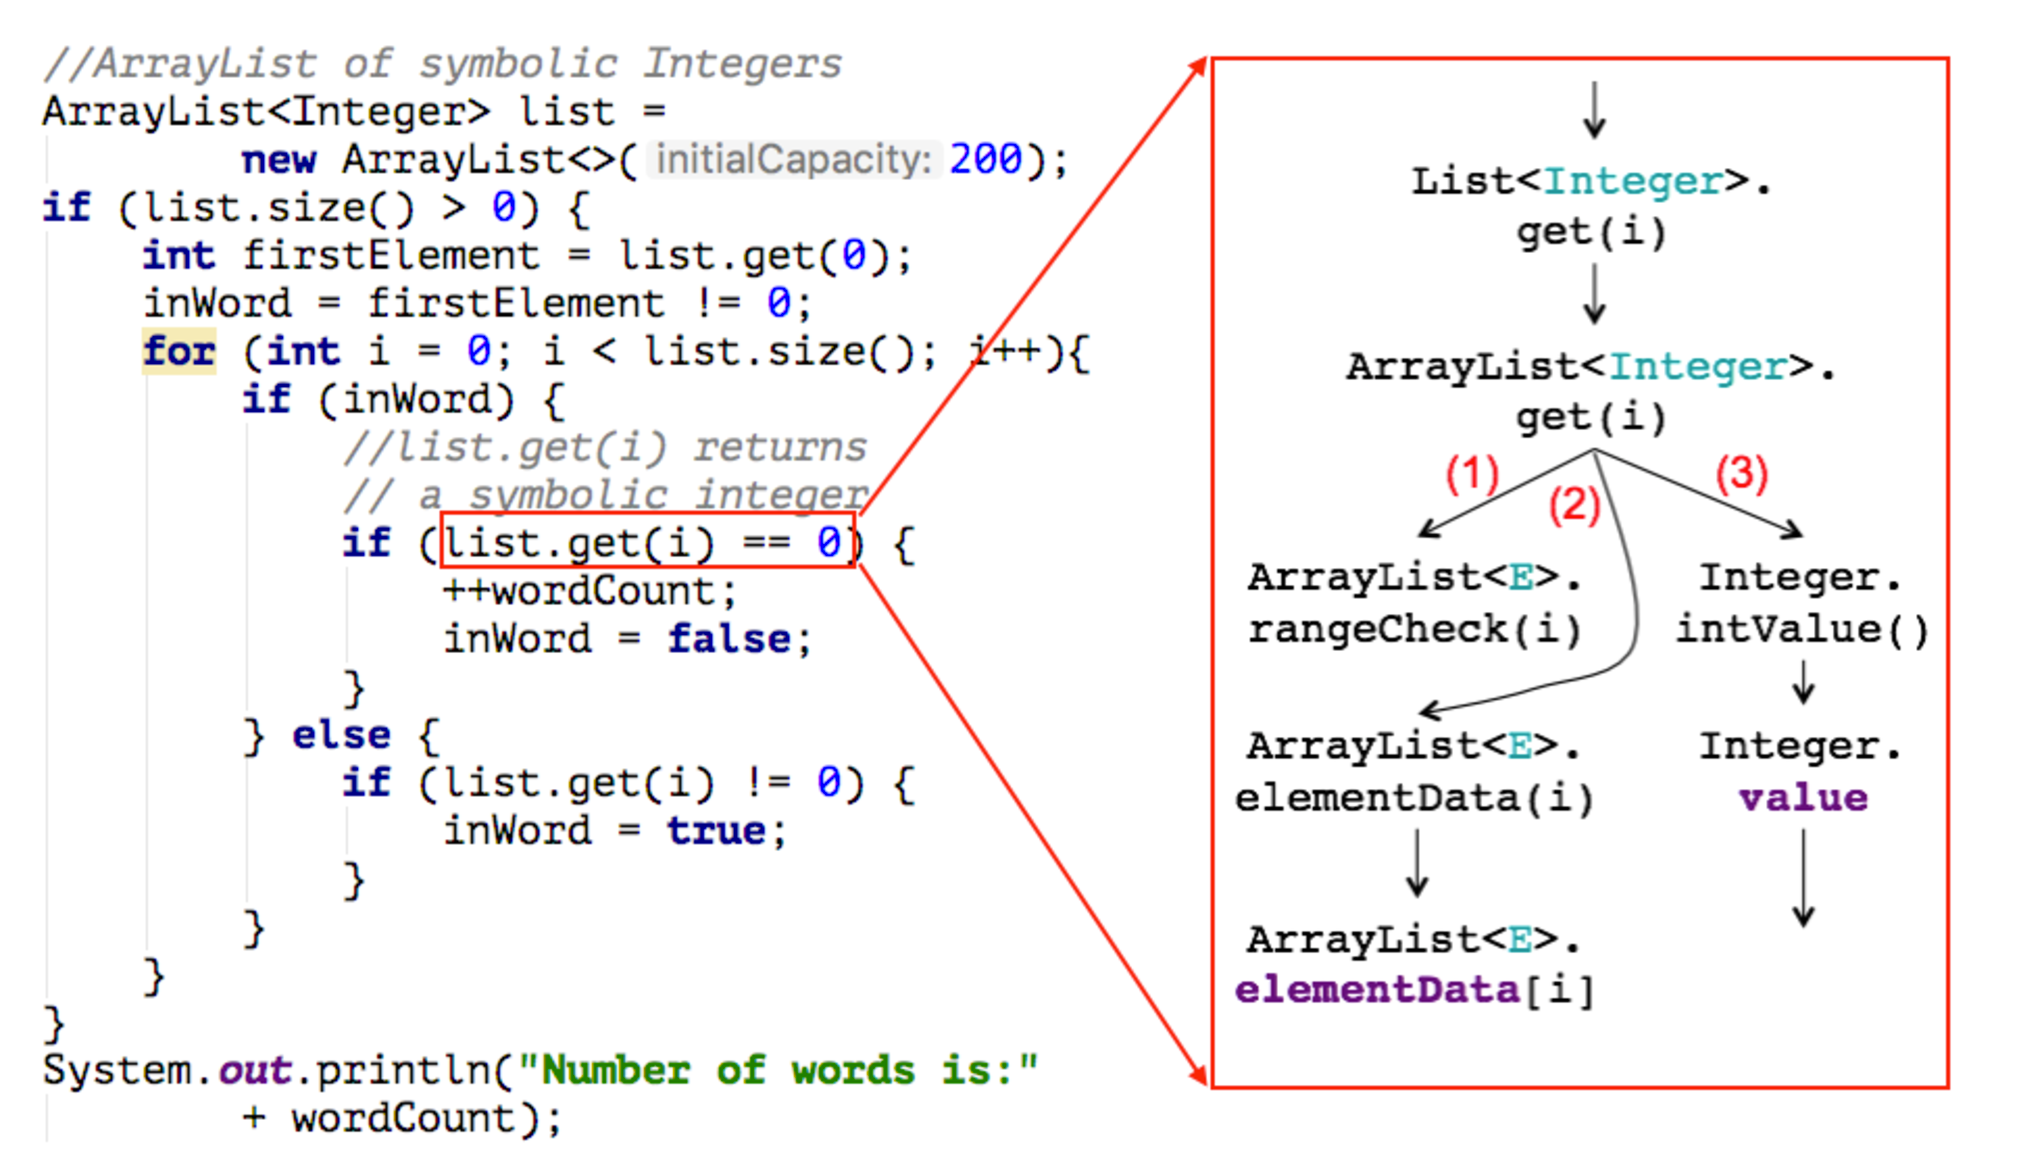
\includegraphics[width=0.8\textwidth]{figures/wordCount.pdf}
    \caption{An example demonstrating the need for using a multi-path region summary}
    \label{fig:mot-example}
\end{figure*}
Consider the example of Java code shown in Figure \ref{fig:mot-example}. The example is used to count number of words where characters are represented with 1 and 0 represents space. 
%
The {\tt list} object refers to an {\tt ArrayList} of 200 {\tt Integer} objects which have an unconstrained symbolic
integer as a field. Checking the first element to be a zero or one introduces a symbolic branch, that requires the symbolic execution to explore both paths. Therefore loop checking for each indexed entry in {\tt list} introduces a branch, which has both sides feasible and which requires the symbolic execution to explore both paths again. \\
%
Performing this check over the entire {\tt list} makes symbolic execution need $2^{100}$ execution paths to terminate
(assuming {\tt list} has 200 entries with every even-indexed entry pointing to a new unconstrained symbolic integer).
%
A simple way to avoid this path explosion is to merge the two paths arising out of the {\tt list.get(i) == 0} branch.
%
Such path merging requires us to compute a summary of all behaviors arising on both sides of the branch of the if-statement inside the for loop.
%
If we can construct such a summary beforehand, our symbolic executor can instantiate the summary by reading in inputs to
the summary from the stack and/or the heap, and writing outputs of the summary to the stack and/or the heap.\\
%
Unfortunately, constructing such a summary for this simple region is not straightforward due to the
call to {\tt list.get(int)} which is actually a call to {\tt ArrayList<Integer>.get(int)} ({\tt java.util.List<E>.get(int)} is abstract and does not have an implementation).
%
{\tt ArrayList<Integer>.get(int)} internally does the following:
%
\begin{enumerate}
\item It checks if the index argument accesses a value within bounds of the {\tt ArrayList} by calling {\tt ArrayList<E>.rangeCheck(int)}. If this access is not within bounds, it throws an exception.
%
\item It calls {\tt ArrayList<E>.elementData(int)} to access an internal array named {\tt elementData} and get the entry at position {\tt i}. This call results in an object of class {\tt Integer} being returned.
%
\item It calls {\tt Integer.intValue()} on the object returned by the previous step. This call internally accesses the {\tt value} field of {\tt Integer} to return the integer value of this object.
%
\end{enumerate}

The static summary of {\tt ArrayList<Integer>.get(int)} needs to not only include summaries of all these three methods but
also include the possibility of an exception being raised by the included summary of {\tt ArrayList<E>.rangeCheck(i)}.
%
Our extension to path-merging includes using method summaries, either with a single return or no return, as part of region summaries that have method calls \footnote{We plan to support methods with multiple returns in the future.}.
%
The method whose summary is to be included depends on the dynamic type of the object reference on which the method is being invoked.
%
In our example, the dynamic type of {\tt list} is {\tt ArrayList}, whereas it is declared statically as having the type {\tt List}.
%
Therefore, the summary of {\tt list.get(i)} pulls in the method summaryof {\tt ArrayList<E>.get(i)}.\\
%
Our \textit{Single-Path Cases} extension to path-merging also allows the possibility of exceptional behavior being
included in the summary and explored separately from unexceptional behavior by performing exploration of exceptional
behavior in the region on its own execution path.\\

We will use this example throughout the reset of the paper to show how different transformations changes the region of interest until a summarization of the region is obtained. 
%
